\documentclass[a4paper,10pt]{article}
\usepackage[english]{babel}
%Includes "References" in the table of contents
\usepackage[nottoc]{tocbibind}
%%
\usepackage{graphicx}
\graphicspath{{./Figures/}}

%\usepackage{subcaption}
%\captionsetup[table]{font=small,size=smaller,textfont=sc}
%\captionsetup[figure]{font=small,size=smaller}

\usepackage{booktabs}
\usepackage{tabularx} %JEA inserted
%\usepackage[T1]{fontenc}
%\usepackage{cite}
%\usepackage[cmex10]{amsmath}
%\usepackage{color}
%\usepackage{bm,bbm}
%\usepackage{wasysym}
%\usepackage{texnames}
%\usepackage{url}

\usepackage[boxed]{algorithm2e}   % AAB inserido
%\usepackage{natbib} % AAB Inserted
\usepackage[listings]{tcolorbox}

%\usepackage{siunitx}
\usepackage{natbib}
\usepackage{multirow,bigstrut}
\usepackage{subfig} % AAB inserted	
\usepackage{booktabs} % AAB inserted
%\usepackage[detect-weight=true, binary-units=true]{siunitx} % AAB inserted
\usepackage{siunitx} % AAB inserted
\usepackage{tikz}  % AAB inserido
\usetikzlibrary{shapes,arrows,shadows}  % AAB inserido
\usepackage{bbm}
%%

%DIF PREAMBLE EXTENSION ADDED BY LATEXDIFF
%DIF UNDERLINE PREAMBLE %DIF PREAMBLE
\RequirePackage[normalem]{ulem} %DIF PREAMBLE
\RequirePackage{color}\definecolor{RED}{rgb}{1,0,0}\definecolor{BLUE}{rgb}{0,0,1} %DIF PREAMBLE
\providecommand{\DIFadd}[1]{{\protect\color{blue}\uwave{#1}}} %DIF PREAMBLE
\providecommand{\DIFdel}[1]{{\protect\color{red}\sout{#1}}}                      %DIF PREAMBLE
%DIF SAFE PREAMBLE %DIF PREAMBLE
\providecommand{\DIFaddbegin}{} %DIF PREAMBLE
\providecommand{\DIFaddend}{} %DIF PREAMBLE
\providecommand{\DIFdelbegin}{} %DIF PREAMBLE
\providecommand{\DIFdelend}{} %DIF PREAMBLE
\providecommand{\DIFmodbegin}{} %DIF PREAMBLE
\providecommand{\DIFmodend}{} %DIF PREAMBLE
%DIF FLOATSAFE PREAMBLE %DIF PREAMBLE
\providecommand{\DIFaddFL}[1]{\DIFadd{#1}} %DIF PREAMBLE
\providecommand{\DIFdelFL}[1]{\DIFdel{#1}} %DIF PREAMBLE
\providecommand{\DIFaddbeginFL}{} %DIF PREAMBLE
\providecommand{\DIFaddendFL}{} %DIF PREAMBLE
\providecommand{\DIFdelbeginFL}{} %DIF PREAMBLE
\providecommand{\DIFdelendFL}{} %DIF PREAMBLE
\newcommand{\DIFscaledelfig}{0.5}
%DIF HIGHLIGHTGRAPHICS PREAMBLE %DIF PREAMBLE
\RequirePackage{settobox} %DIF PREAMBLE
\RequirePackage{letltxmacro} %DIF PREAMBLE
\newsavebox{\DIFdelgraphicsbox} %DIF PREAMBLE
\newlength{\DIFdelgraphicswidth} %DIF PREAMBLE
\newlength{\DIFdelgraphicsheight} %DIF PREAMBLE
% store original definition of \includegraphics %DIF PREAMBLE
\LetLtxMacro{\DIFOincludegraphics}{\includegraphics} %DIF PREAMBLE
\newcommand{\DIFaddincludegraphics}[2][]{{\color{blue}\fbox{\DIFOincludegraphics[#1]{#2}}}} %DIF PREAMBLE
\newcommand{\DIFdelincludegraphics}[2][]{% %DIF PREAMBLE
\sbox{\DIFdelgraphicsbox}{\DIFOincludegraphics[#1]{#2}}% %DIF PREAMBLE
\settoboxwidth{\DIFdelgraphicswidth}{\DIFdelgraphicsbox} %DIF PREAMBLE
\settoboxtotalheight{\DIFdelgraphicsheight}{\DIFdelgraphicsbox} %DIF PREAMBLE
\scalebox{\DIFscaledelfig}{% %DIF PREAMBLE
	\parbox[b]{\DIFdelgraphicswidth}{\usebox{\DIFdelgraphicsbox}\\[-\baselineskip] \rule{\DIFdelgraphicswidth}{0em}}\llap{\resizebox{\DIFdelgraphicswidth}{\DIFdelgraphicsheight}{% %DIF PREAMBLE
			\setlength{\unitlength}{\DIFdelgraphicswidth}% %DIF PREAMBLE
			\begin{picture}(1,1)% %DIF PREAMBLE
			\thicklines\linethickness{2pt} %DIF PREAMBLE
			{\color[rgb]{1,0,0}\put(0,0){\framebox(1,1){}}}% %DIF PREAMBLE
			{\color[rgb]{1,0,0}\put(0,0){\line( 1,1){1}}}% %DIF PREAMBLE
			{\color[rgb]{1,0,0}\put(0,1){\line(1,-1){1}}}% %DIF PREAMBLE
			\end{picture}% %DIF PREAMBLE
		}\hspace*{3pt}}} %DIF PREAMBLE
} %DIF PREAMBLE
\LetLtxMacro{\DIFOaddbegin}{\DIFaddbegin} %DIF PREAMBLE
\LetLtxMacro{\DIFOaddend}{\DIFaddend} %DIF PREAMBLE
\LetLtxMacro{\DIFOdelbegin}{\DIFdelbegin} %DIF PREAMBLE
\LetLtxMacro{\DIFOdelend}{\DIFdelend} %DIF PREAMBLE
\DeclareRobustCommand{\DIFaddbegin}{\DIFOaddbegin \let\includegraphics\DIFaddincludegraphics} %DIF PREAMBLE
\DeclareRobustCommand{\DIFaddend}{\DIFOaddend \let\includegraphics\DIFOincludegraphics} %DIF PREAMBLE
\DeclareRobustCommand{\DIFdelbegin}{\DIFOdelbegin \let\includegraphics\DIFdelincludegraphics} %DIF PREAMBLE
\DeclareRobustCommand{\DIFdelend}{\DIFOaddend \let\includegraphics\DIFOincludegraphics} %DIF PREAMBLE
\LetLtxMacro{\DIFOaddbeginFL}{\DIFaddbeginFL} %DIF PREAMBLE
\LetLtxMacro{\DIFOaddendFL}{\DIFaddendFL} %DIF PREAMBLE
\LetLtxMacro{\DIFOdelbeginFL}{\DIFdelbeginFL} %DIF PREAMBLE
\LetLtxMacro{\DIFOdelendFL}{\DIFdelendFL} %DIF PREAMBLE
\DeclareRobustCommand{\DIFaddbeginFL}{\DIFOaddbeginFL \let\includegraphics\DIFaddincludegraphics} %DIF PREAMBLE
\DeclareRobustCommand{\DIFaddendFL}{\DIFOaddendFL \let\includegraphics\DIFOincludegraphics} %DIF PREAMBLE
\DeclareRobustCommand{\DIFdelbeginFL}{\DIFOdelbeginFL \let\includegraphics\DIFdelincludegraphics} %DIF PREAMBLE
\DeclareRobustCommand{\DIFdelendFL}{\DIFOaddendFL \let\includegraphics\DIFOincludegraphics} %DIF PREAMBLE
%DIF LISTINGS PREAMBLE %DIF PREAMBLE
\RequirePackage{listings} %DIF PREAMBLE
\RequirePackage{color} %DIF PREAMBLE
\lstdefinelanguage{DIFcode}{ %DIF PREAMBLE
%DIF DIFCODE_UNDERLINE %DIF PREAMBLE
moredelim=[il][\color{red}\sout]{\%DIF\ <\ }, %DIF PREAMBLE
moredelim=[il][\color{blue}\uwave]{\%DIF\ >\ } %DIF PREAMBLE
} %DIF PREAMBLE
\lstdefinestyle{DIFverbatimstyle}{ %DIF PREAMBLE
language=DIFcode, %DIF PREAMBLE
basicstyle=\ttfamily, %DIF PREAMBLE
columns=fullflexible, %DIF PREAMBLE
keepspaces=true %DIF PREAMBLE
} %DIF PREAMBLE
\lstnewenvironment{DIFverbatim}{\lstset{style=DIFverbatimstyle}}{} %DIF PREAMBLE
\lstnewenvironment{DIFverbatim*}{\lstset{style=DIFverbatimstyle,showspaces=true}}{} %DIF PREAMBLE
%DIF END PREAMBLE EXTENSION ADDED BY LATEXDIFF
%%

%Title, date an author of the document
\title{Bibliography management: BibTeX}
\author{Overleaf}

%Begining of the document
\begin{document}

%%% AAB - Mudei o titulo
\title{Fast Noise Reduction in InSAR Data with Empirical Statistical Models\\
	Revision R1}


\author{Anderson A.\ De Borba,
	Joselito E.\ De Araújo, and
	Alejandro C. Frery}


\maketitle


\section{Review Report}
\begin{tcolorbox}[colback=red!5!white,colframe=red!75!black,title=Review Report]
This manuscript addresses an important topic in InSAR phase filtering, namely the trade-off between denoising performance and computational efficiency. The paper proposes three filters, LInSARRFE, TcNfilter, and TcCfilter, and evaluates them on
simulated and real InSAR datasets. The topic is relevant, and the results suggest
substantial runtime savings with competitive filtering accuracy. However, several
issues should be addressed before the manuscript can be considered for publication.

1. The literature review still needs improvement. For example, in terms of
InSAR applications, it should cover land subsidence susceptibility mapping(He, Y.,
Gao, B., Yan, H., Zhang, Q., Zhang, L., Li, W., He, X., Lu, J. DBPFNet: A double
branch parallel fusion neural network method for land subsidence susceptibility
mapping with InSAR observation data. International Journal of Digital Earth, 2025,
18(1): 2499199.) and ground deformation prediction(Wang, J., Hu, J., Zhou, Z. et al.
Integrating Explainable Machine Learning and LSTM with Multiple Factors for
Mechanism Identification and Prediction of Land Deformation in the North Henan
Plain. J geovis spat anal 10, 5 (2026). https://doi.org/10.1007/s41651-025-00246-z).

2. The novelty should be stated more clearly.The manuscript proposes three
filters and emphasizes their computational advantages, but the distinction between a
genuinely new methodological contribution and an implementation-level modification
of the Refined Lee framework remains somewhat unclear. The paper should better
clarify what is fundamentally new in LInSARRFE, TcNfilter, and TcCfilter, and how
these methods differ conceptually from the existing physical and empirical models
discussed in the introduction.

3. The comparative evaluation is too limited.At present, the main benchmark is
the Refined Lee filter, which the authors use as the state-of-the-art reference. However,
the introduction itself acknowledges that InSAR phase filtering methods include
spatial-domain, transform-domain, and non-local approaches. The manuscript would
be much stronger if the proposed methods were also compared with at least one
representative transform-domain method and one non-local method, rather than only
with Refined Lee.

4. A statistical significance analysis is missing.The manuscript reports
performance differences in terms of RMSE, SSIM, residual reduction, and runtime,
but it is unclear whether the simulated experiments were repeated multiple times with
different random seeds or noise realizations. Reporting only single values makes it
difficult to assess the robustness of the observed gains. The authors should report
mean ± standard deviation and, if possible, include significance testing for the key
performance comparisons.

5. An ablation analysis would help explain where the performance gains come
from. The proposed methods involve several changes simultaneously, including
empirical models, directional window selection, and MMSE-based estimation within
the filtering framework. It is therefore difficult to determine which design choice
contributes most to the final improvement. An ablation study would be useful, for
example by isolating the effect of the empirical model replacement from the effect of
the directional window strategy.
\end{tcolorbox}

\begin{tcolorbox}[colback=red!5!white,colframe=red!75!black,title=Review Report continuation.]
6. The conclusions regarding Sentinel-1 versus UAVSAR should be stated more
cautiously. The manuscript suggests that Sentinel-1 data show systematically better
residual reduction and computational performance than UAVSAR data, and further
suggests that Sentinel-1 may better match the assumptions of the proposed models.
This interpretation may be reasonable, but it is based on a limited number of case
studies and may also be influenced by differences in acquisition conditions, scene
characteristics, or resolution. The conclusion should therefore be toned down unless
additional evidence is provided.

7. It is suggested that Figure 3 be moved to Sections 2.1.2–2.1.4, where it would
better match the corresponding content and improve the logical flow of the
manuscript. Moreover, adding remote sensing satellite imagery and/or field
photographs would help readers better understand the study area and enhance the
overall presentation of the paper.
8. In Figure 10-12, d) TcNfilter should be (d).
\end{tcolorbox}

%%%%%%%%%%%%%%%%%%%%%%%%%%%%%%%%%%%%%%%%%%%%%%%%%%%%%%%%%%%%%%%%%%%%%%%%%%%%%%%%%%
%%%%%%%%%%%%%%%%%%%%%%%%%%% Comment #1 %%%%%%%%%%%%%%%%%%%%%%%%%%%%%%%%%%%%%%%%%%%
%%%%%%%%%%%%%%%%%%%%%%%%%%%%%%%%%%%%%%%%%%%%%%%%%%%%%%%%%%%%%%%%%%%%%%%%%%%%%%%%%%


\section{Answers to Reviewer. \#1}

Thank you very much for handling this manuscript.

We have prepared a revised version taking into account all the comments and suggestions made.

In fact, we found the review well-informed and constructive. We would like to thank the reviewer.

This response letter addresses all the comments in red, followed by
our reactions, and, whenever necessary, the changes made.

The authors

\vskip3em\begin{tcolorbox}[colback=red!5!white,colframe=red!75!black,title=Comment 1]
% AAB inserido
1. The literature review still needs improvement. For example, in terms of
InSAR applications, it should cover land subsidence susceptibility mapping(He, Y.,
Gao, B., Yan, H., Zhang, Q., Zhang, L., Li, W., He, X., Lu, J. DBPFNet: A double
branch parallel fusion neural network method for land subsidence susceptibility
mapping with InSAR observation data. International Journal of Digital Earth, 2025,
18(1): 2499199.) and ground deformation prediction(Wang, J., Hu, J., Zhou, Z. et al.
Integrating Explainable Machine Learning and LSTM with Multiple Factors for
Mechanism Identification and Prediction of Land Deformation in the North Henan
Plain. J geovis spat anal 10, 5 (2026). https://doi.org/10.1007/s41651-025-00246-z).
\end{tcolorbox}

\begin{tcolorbox}[colback=white,colframe=black,title=Changes 1]
We have added those references in a new category of phase denoising.
\end{tcolorbox}


%%%%%%%%%%%%%%%%%%%%%%%%%%%%%%%%%%%%%%%%%%%%%%%%%%%%%%%%%%%%%%%%%%%%%%%%%%%%%%%%%%
%%%%%%%%%%%%%%%%%%%%%%%%%%% Comment #2 %%%%%%%%%%%%%%%%%%%%%%%%%%%%%%%%%%%%%%%%%%%
%%%%%%%%%%%%%%%%%%%%%%%%%%%%%%%%%%%%%%%%%%%%%%%%%%%%%%%%%%%%%%%%%%%%%%%%%%%%%%%%%%
\vskip3em\begin{tcolorbox}[colback=red!5!white,colframe=red!75!black,title=Comment 2]
2. The novelty should be stated more clearly.The manuscript proposes three
filters and emphasizes their computational advantages, but the distinction between a
genuinely new methodological contribution and an implementation-level modification
of the Refined Lee framework remains somewhat unclear. The paper should better
clarify what is fundamentally new in LInSARRFE, TcNfilter, and TcCfilter, and how
these methods differ conceptually from the existing physical and empirical models
discussed in the introduction.
\end{tcolorbox}

\begin{tcolorbox}[colback=white,colframe=black,title=Changes 2]
We reshaped our introduction to better reflect our contribution.
\end{tcolorbox}



%%%%%%%%%%%%%%%%%%%%%%%%%%%%%%%%%%%%%%%%%%%%%%%%%%%%%%%%%%%%%%%%%%%%%%%%%%%%%%%%%%
%%%%%%%%%%%%%%%%%%%%%%%%%%% Comment #3 %%%%%%%%%%%%%%%%%%%%%%%%%%%%%%%%%%%%%%%%%%%
%%%%%%%%%%%%%%%%%%%%%%%%%%%%%%%%%%%%%%%%%%%%%%%%%%%%%%%%%%%%%%%%%%%%%%%%%%%%%%%%%%
\vskip3em\begin{tcolorbox}[colback=red!5!white,colframe=red!75!black,title=Comment 3]
3. The comparative evaluation is too limited. At present, the main benchmark is
the Refined Lee filter, which the authors use as the state-of-the-art reference. However,
the introduction itself acknowledges that InSAR phase filtering methods include
spatial-domain, transform-domain, and non-local approaches. The manuscript would
be much stronger if the proposed methods were also compared with at least one
representative transform-domain method and one non-local method, rather than only
with Refined Lee.

\end{tcolorbox}

\begin{tcolorbox}[colback=white,colframe=black,title=Changes 3]
While we appreciate the reviewer’s suggestion, we wish to emphasize that the novelty of this research does not stem from improved denoising over previous filters, but rather from the optimization of the underlying model with execution speed in mind.
The new introduction makes this clear.
This approach allows for substantial reductions in processing time while maintaining the high standards of result quality expected from established techniques. 
Because our contribution is centered on this structural replacement and its subsequent efficiency gains, we prefer to exclude comparisons with filters from different domains, as such metrics would not accurately reflect the specific modeling advancements achieved in this research.
\end{tcolorbox}


%%%%%%%%%%%%%%%%%%%%%%%%%%%%%%%%%%%%%%%%%%%%%%%%%%%%%%%%%%%%%%%%%%%%%%%%%%%%%%%%%%
%%%%%%%%%%%%%%%%%%%%%%%%%%% Comment #4 %%%%%%%%%%%%%%%%%%%%%%%%%%%%%%%%%%%%%%%%%%%
%%%%%%%%%%%%%%%%%%%%%%%%%%%%%%%%%%%%%%%%%%%%%%%%%%%%%%%%%%%%%%%%%%%%%%%%%%%%%%%%%%
\vskip3em\begin{tcolorbox}[colback=red!5!white,colframe=red!75!black,title=Comment 4]

4. A statistical significance analysis is missing.The manuscript reports
performance differences in terms of RMSE, SSIM, residual reduction, and runtime,
but it is unclear whether the simulated experiments were repeated multiple times with
different random seeds or noise realizations. Reporting only single values makes it
difficult to assess the robustness of the observed gains. The authors should report
mean ± standard deviation and, if possible, include significance testing for the key
performance comparisons.

\end{tcolorbox}

\begin{tcolorbox}[colback=white,colframe=black,title=Changes 4]
Thank you very much for your contribution. The authors fully agree with the suggestion, and we have made the following modification in the Simulated InSAR Data:

As shown in Table~\ref{TabEficiencia_simu}, the TcCfilter exhibits the lowest \DIFaddbegin \DIFadd{mean }\DIFaddend RMSE and the highest accuracy among the analyzed filters \DIFaddbegin \DIFadd{across the $R = 30$ noise realizations}\DIFaddend . Additionally, the proposed filters LInSARRFE and TcNfilter present \DIFaddbegin \DIFadd{mean }\DIFaddend RMSE values that are only slightly higher than those of the Refined Lee filter.

\begin{center}
	\captionof{table}{Efficiency of filters for simulated data: mean $\pm$ standard deviation over $R = 30$ independent noise realizations. Runtime (RT) values correspond to the average time among all replications. Time savings are computed relative to Ref.\ Lee and bold entries indicate the best value per column.\label{TabEficiencia_simu}}
	\begin{tabularx}{\textwidth}{
			l
			>{\centering\arraybackslash}X
			>{\centering\arraybackslash}X
			r
			>{\centering\arraybackslash}X
		}
		\toprule
		\textbf{Filter} & \textbf{RMSE (mean $\pm$ sd)} & \textbf{SSIM (mean $\pm$ sd)} & \textbf{RT (s)} & \textbf{Time Saved (\%)}\\
		\midrule
		Ref. Lee  & $\mathbf{1.84038 \pm 6.8\cdot 10^{-3}}$ & $\mathbf{0.945286 \pm 4.1\cdot 10^{-4}}$ & 5656.09 & $\text{---}$ \\
		LInSARRFE & ${1.84926 \pm 4.7\cdot 10^{-3}}$         & ${0.944787 \pm 2.8\cdot 10^{-4}}$         & 624.82  & 88.95 \\
		TcNfilter & ${1.879114 \pm 6.6\cdot 10^{-3}}$        & ${0.943092 \pm 3.9\cdot 10^{-4}}$         & $\mathbf{343.78}$ & $\mathbf{93.92}$ \\
		TcCfilter & ${1.849049 \pm 4.6\cdot 10^{-3}}$        & ${0.944799 \pm 2.7\cdot 10^{-4}}$         & 433.64  & 92.33 \\
		\bottomrule
	\end{tabularx}
\end{center}

\DIFaddbegin \DIFadd{The Kruskal--Wallis test applied to the 30-replication RMSE distributions yields a statistically significant result (H:
   $H_0$: All distributions are equal (medians are equal across filters),
   $H_1$: At least one distribution differs, $\text{df} = 3$, $p=0.000001 < 0.05$), confirming that the filters differ in their denoising accuracy.
   }

\DIFadd{Pairwise Wilcoxon signed-rank tests
 (H: $H_0$: The filter distribution is the same as Ref. Lee's
  $H_1$: The distributions differ)
against the Ref.\ Lee baseline (Bonferroni-corrected at $\alpha_{\text{adj}} = 0.01667$) show that TcCfilter achieves a significantly lower RMSE ($p=0.000002 < 0.017$), and LInSARRFE and TcNfilter show similar results.
All alternative filters differ significantly from Ref. Lee's for RMSE and SSIM.
}

\DIFaddend Regarding SSIM, the metric that evaluates the structural similarity between the filtered interferogram and the reference image (noise-free)~\cite{ANonlocalFilterforSARInterferometric}, the Refined Lee filter shows a slight advantage, with a value closer to $1$. 
The proposed filters, especially LInSARRFE and TcCfilter, exhibit SSIM values very close to those of the Refined Lee filter, indicating no significant loss in preserving image structure. 

Regarding runtime, the proposed filters significantly outperform the Refined Lee filter, which has the longest processing times, potentially restricting its use in time-sensitive applications. 
Notably, the TcNfilter achieves the greatest time savings, resulting in an approximate time reduction of 
\DIFdelbegin \DIFdel{\mbox{%DIFAUXCMD
\qty{92}{\percent}}\hskip0pt%DIFAUXCMD
}\DIFdelend \DIFaddbegin \DIFadd{\mbox{%DIFAUXCMD
\qty{93.92}{\percent}}\hskip0pt%DIFAUXCMD
}\DIFaddend . 
In contrast, the slow processing of the Refined Lee filter limits its practical applicability. 
Therefore, the proposed filters excel over the Refined Lee filter in terms of \DIFdelbegin \DIFdel{accuracy, structural preservation, and }\DIFdelend processing efficiency.
\end{tcolorbox}


%%%%%%%%%%%%%%%%%%%%%%%%%%%%%%%%%%%%%%%%%%%%%%%%%%%%%%%%%%%%%%%%%%%%%%%%%%%%%%%%%%
%%%%%%%%%%%%%%%%%%%%%%%%%%% Comment #5 %%%%%%%%%%%%%%%%%%%%%%%%%%%%%%%%%%%%%%%%%%%
%%%%%%%%%%%%%%%%%%%%%%%%%%%%%%%%%%%%%%%%%%%%%%%%%%%%%%%%%%%%%%%%%%%%%%%%%%%%%%%%%%
\vskip3em\begin{tcolorbox}[colback=red!5!white,colframe=red!75!black,title=Comment 5]
5. An ablation analysis would help explain where the performance gains come
from. The proposed methods involve several changes simultaneously, including
empirical models, directional window selection, and MMSE-based estimation within
the filtering framework. It is therefore difficult to determine which design choice
contributes most to the final improvement. An ablation study would be useful, for
example by isolating the effect of the empirical model replacement from the effect of
the directional window strategy.

\end{tcolorbox}

\begin{tcolorbox}[colback=white,colframe=black,title=Changes 5]
We have now clarified that the filters are comparable regarding their execution times because we have fixed as benchmark the Refined Lee filter on top of an adaptive window scheme.
All other filters use the same adaptive window scheme, while changing the statistical model.

\DIFadd{The }\DIFaddend Refined Lee InSAR filter was chosen as the \DIFdelbegin \DIFdel{sole }\DIFdelend benchmark because it’s the \DIFdelbegin \DIFdel{basic }\DIFdelend \DIFaddbegin \DIFadd{widely employed }\DIFaddend spatial-domain statistical filtering method from which both the Enhanced Refined Lee variant and the methods in this work are derived. A \DIFdelbegin \DIFdel{wider }\DIFdelend \DIFaddbegin \DIFadd{broader }\DIFaddend comparison of all Lee filter variants is beyond the scope of this study and \DIFdelbegin \DIFdel{is a potential }\DIFdelend \DIFaddbegin \DIFadd{warrants }\DIFaddend future investigation.


\end{tcolorbox}


%%%%%%%%%%%%%%%%%%%%%%%%%%%%%%%%%%%%%%%%%%%%%%%%%%%%%%%%%%%%%%%%%%%%%%%%%%%%%%%%%%
%%%%%%%%%%%%%%%%%%%%%%%%%%% Comment #6 %%%%%%%%%%%%%%%%%%%%%%%%%%%%%%%%%%%%%%%%%%%
%%%%%%%%%%%%%%%%%%%%%%%%%%%%%%%%%%%%%%%%%%%%%%%%%%%%%%%%%%%%%%%%%%%%%%%%%%%%%%%%%%
\vskip3em\begin{tcolorbox}[colback=red!5!white,colframe=red!75!black,title=Comment 6]
6. The conclusions regarding Sentinel-1 versus UAVSAR should be stated more
cautiously. The manuscript suggests that Sentinel-1 data show systematically better
residual reduction and computational performance than UAVSAR data, and further
suggests that Sentinel-1 may better match the assumptions of the proposed models.
This interpretation may be reasonable, but it is based on a limited number of case
studies and may also be influenced by differences in acquisition conditions, scene
characteristics, or resolution. The conclusion should therefore be toned down unless
additional evidence is provided.

\end{tcolorbox}

\begin{tcolorbox}[colback=white,colframe=black,title=Changes 6]
Thank you very much for your contribution. The authors fully agree with the suggestion, and we have made the following modification in Conclusion section:


\DIFaddbegin \DIFadd{Testing with }\DIFaddend Sentinel-1 data showed \DIFdelbegin \DIFdel{systematically }\DIFdelend greater reductions in phase residuals and better computational performance than UAVSAR data when processed with the proposed methods. \DIFdelbegin \DIFdel{This }\DIFdelend \DIFaddbegin \DIFadd{The above }\DIFaddend suggests that the characteristics of Sentinel-1 data better \DIFdelbegin \DIFdel{match }\DIFdelend \DIFaddbegin \DIFadd{align with }\DIFaddend the assumptions of the proposed \DIFaddbegin \DIFadd{physics-}\DIFaddend statistical and empirical models. \DIFaddbegin \DIFadd{However, further investigation is needed.
}

%DIF > Sentinel-1 data showed systematically greater reductions in phase residuals and better computational performance than UAVSAR data when processed with the proposed methods. 
%DIF > This suggests that the characteristics of Sentinel-1 data better match the assumptions of the proposed statistical and empirical models. 
\DIFaddend However, further investigation is needed.

\end{tcolorbox}


%%%%%%%%%%%%%%%%%%%%%%%%%%%%%%%%%%%%%%%%%%%%%%%%%%%%%%%%%%%%%%%%%%%%%%%%%%%%%%%%%%
%%%%%%%%%%%%%%%%%%%%%%%%%%% Comment #7 %%%%%%%%%%%%%%%%%%%%%%%%%%%%%%%%%%%%%%%%%%%
%%%%%%%%%%%%%%%%%%%%%%%%%%%%%%%%%%%%%%%%%%%%%%%%%%%%%%%%%%%%%%%%%%%%%%%%%%%%%%%%%%
\vskip3em\begin{tcolorbox}[colback=red!5!white,colframe=red!75!black,title=Comment 7]
7. It is suggested that Figure 3 be moved to Sections 2.1.2–2.1.4, where it would
better match the corresponding content and improve the logical flow of the
manuscript. Moreover, adding remote sensing satellite imagery and/or field
photographs would help readers better understand the study area and enhance the
overall presentation of the paper.
\end{tcolorbox}


\begin{tcolorbox}[colback=white,colframe=black,title=Changes 7]

Thank you very much for your contribution. The authors fully agree with the suggestion, and we have made the following modification in 2.1.3 e 2.1.4  sections:

%DIFDELCMD < %%%
\DIFdelend We analyzed data from the eruption of the La Cumbre volcano on Fernandina Island in the Galápagos archipelago, Ecuador, on January 12, 2020, see~\cite{pechnikovLaCumbre}.  The Region of Interest (ROI) \DIFaddbegin \DIFadd{of the InSAR image }\DIFaddend presented in Figure~\DIFdelbegin \DIFdel{\ref{fig:insar_la_cumbre:c} }\DIFdelend \DIFaddbegin \DIFadd{\ref{fig:insar_la_cumbre_InSAR} }\DIFaddend has $346\times492$ pixels.

\DIFaddbegin \DIFadd{Figure~\ref{fig:insar_la_cumbre_optica} shows the optical image of the La Cumbre region. Although we did not work with optical images in this research, we know they can show the volcano's characteristics very well and emphasize mountain features. For example, Figure~\ref{fig:insar_la_cumbre_optica} shows that the ground is very sloped closer to the volcano, whereas farther from the volcano is a flat region. The advantage of InSAR images is that they allow us to estimate the volcano's slope and height. In this way, we can monitor several environmental hazards, such as landslide or lava-flow speeds after a volcanic eruption, among many possibilities. The authors emphasized that no coregistration of the images was performed.   
}

\DIFaddend
\end{tcolorbox}

\begin{figure}[hbt]
\centering
	\DIFdelbeginFL %DIFDELCMD < 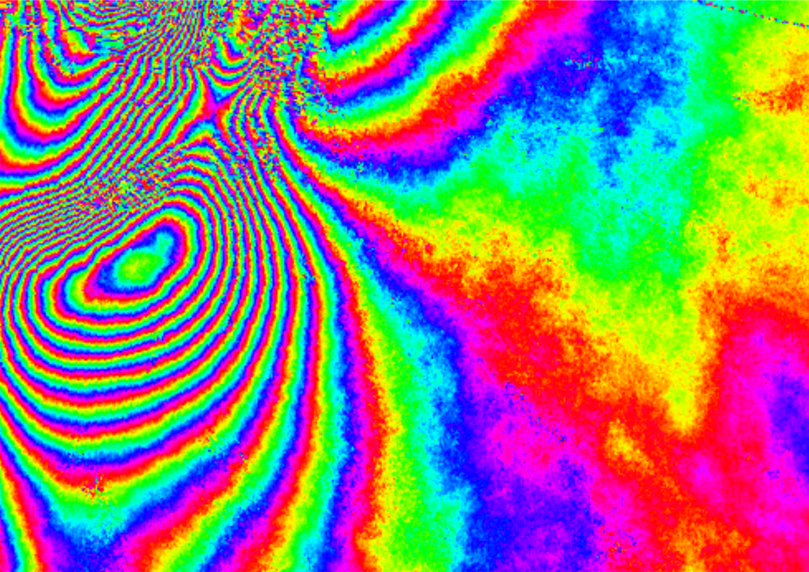
\includegraphics[width=0.567\linewidth]{interferograma_LaCumbe}
%DIFDELCMD < %%%
\DIFdelendFL \DIFaddbeginFL \subfloat[InSAR Image\label{fig:insar_la_cumbre_InSAR}]{
		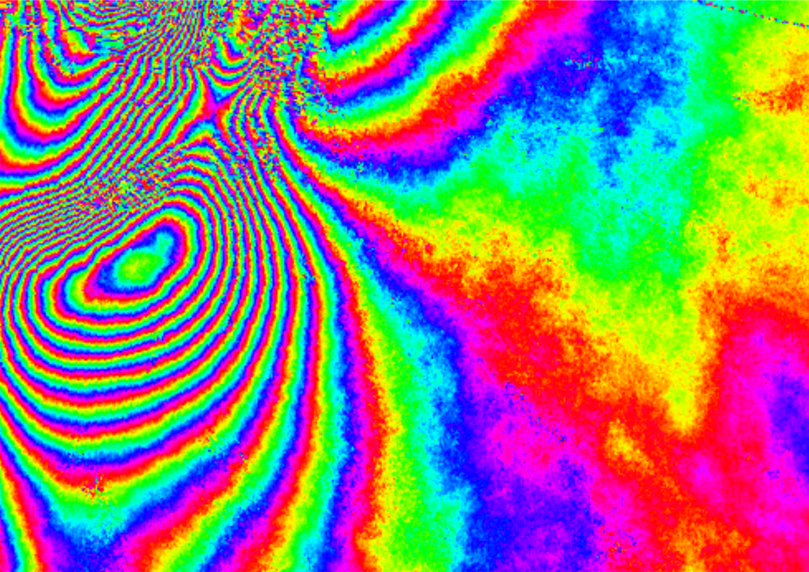
\includegraphics[width=0.5\linewidth]{interferograma_LaCumbe.pdf}}
	\subfloat[Optical Image\label{fig:insar_la_cumbre_optica}]{
		%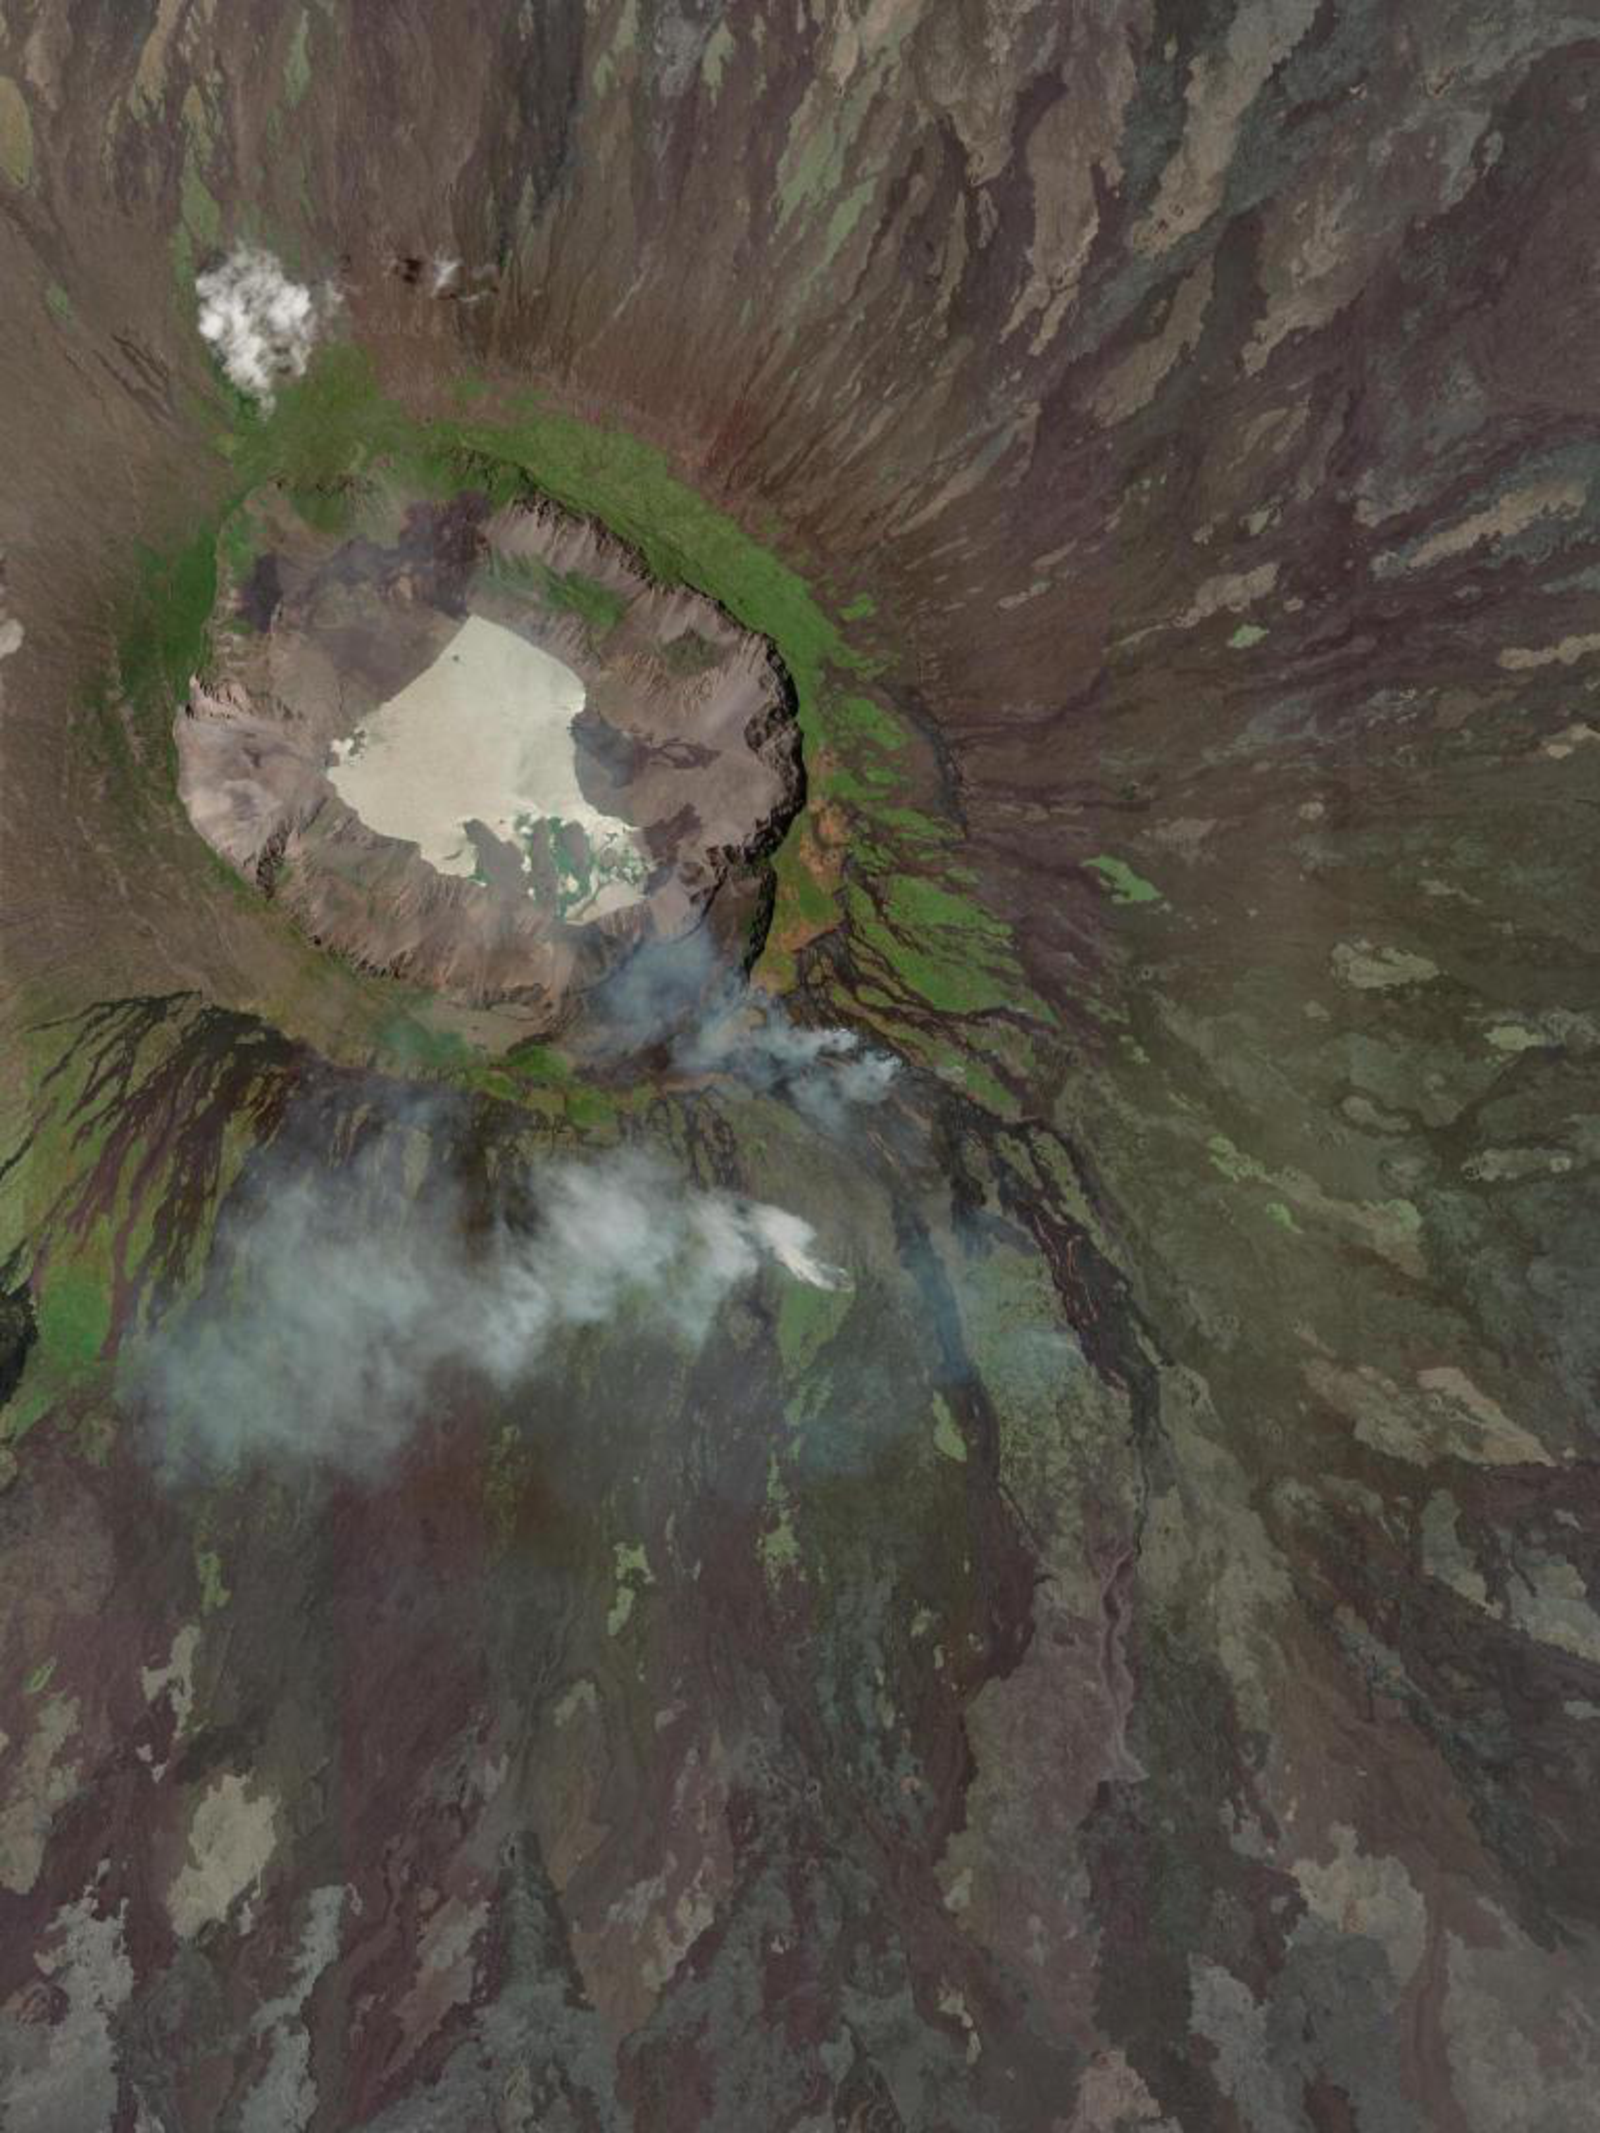
\includegraphics[width=0.265\linewidth]{la_cumbre_high_res.pdf}}
		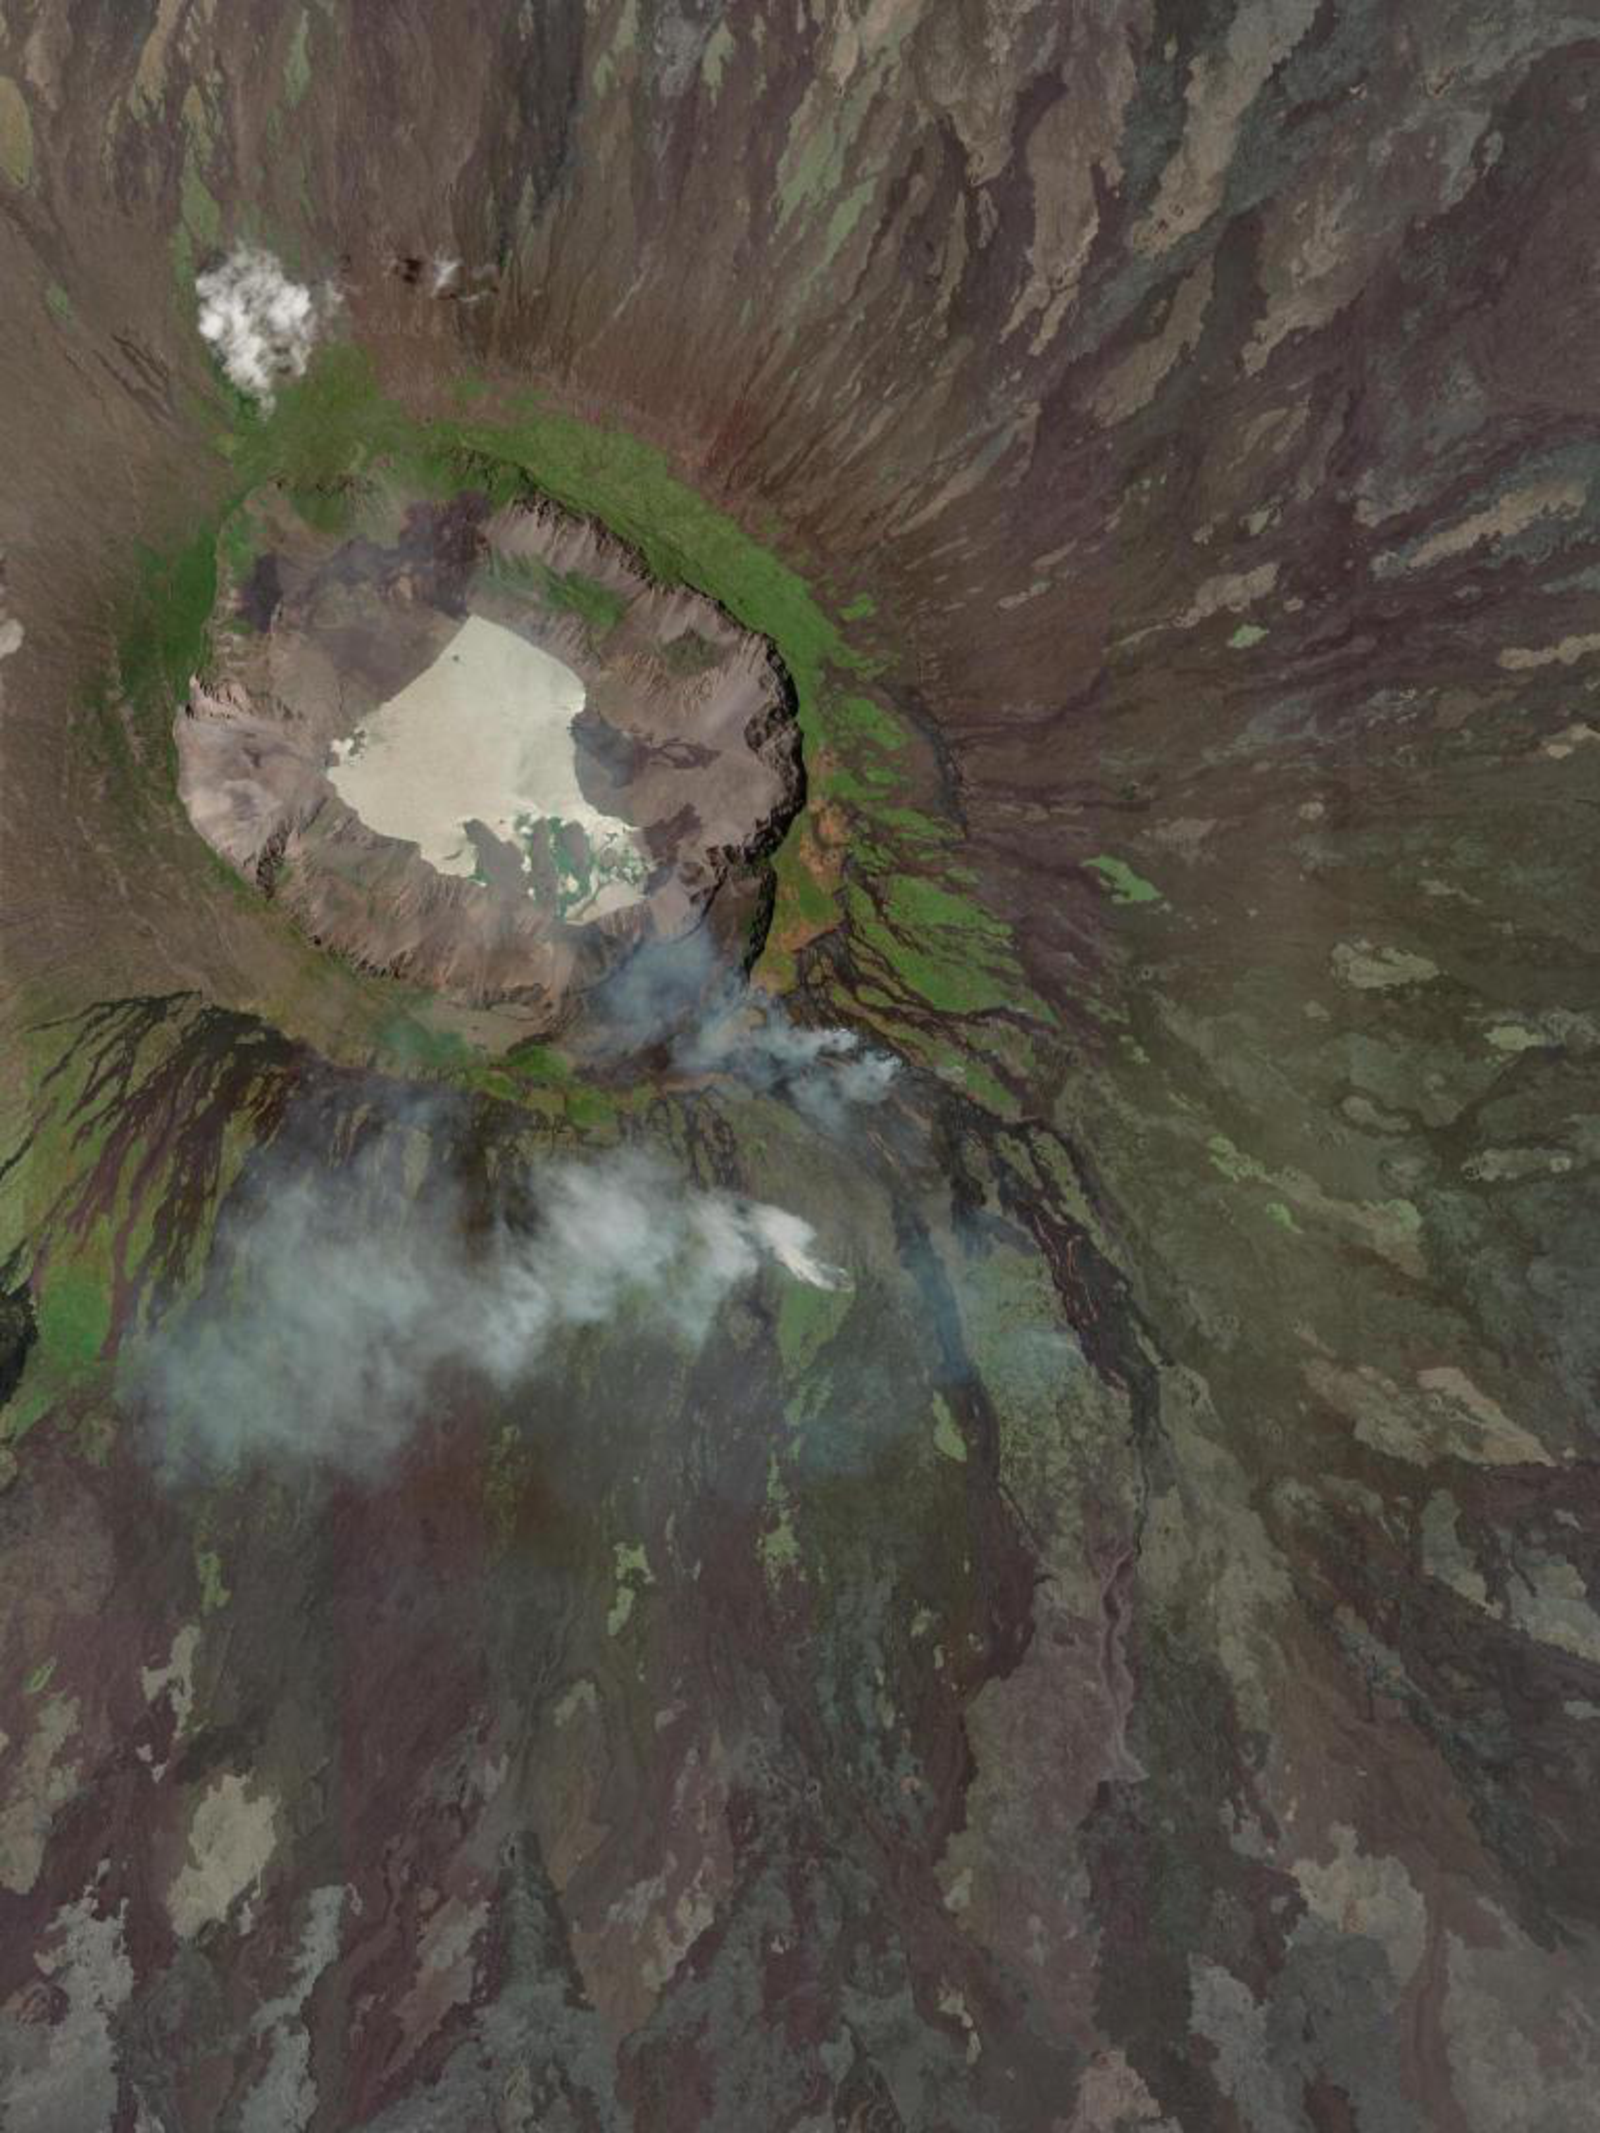
\includegraphics[width=0.48\linewidth, height=4.89cm]{la_cumbre_high_res.pdf}}
	\DIFaddendFL \caption{La Cumbre Volcano \DIFdelbeginFL \DIFdelFL{InSAR Image}\DIFdelendFL \DIFaddbeginFL \DIFaddFL{Images}\DIFaddendFL }
	\DIFdelbeginFL %DIFDELCMD < \label{fig:insar_la_cumbre:c}
%DIFDELCMD < %%%
\DIFdelendFL \DIFaddbeginFL \label{fig:insar_la_cumbre}
\DIFaddendFL \end{figure}


\subsubsection{Los Alamos InSAR Image}\label{subsec:materials_los_alamos}

Figure~\DIFdelbegin \DIFdel{\ref{fig:insar_uavsar_los_alamos:a} }\DIFdelend \DIFaddbegin \DIFadd{\ref{fig:insar_uavsar_los_alamos} }\DIFaddend shows the InSAR image of Los Alamos, USA, to the left, while the right image is the region of interest (ROI) that we use for testing.


\DIFaddbegin \begin{figure}[hbt]    
	\centering
      %DIF >    \subfloat[Los Alamos InSAR Image \label{fig:insar_uavsar_los_alamos:a}]{%
%DIF >        \includegraphics[width=0.52\linewidth]{arquivo_fix_alamos.pdf}
		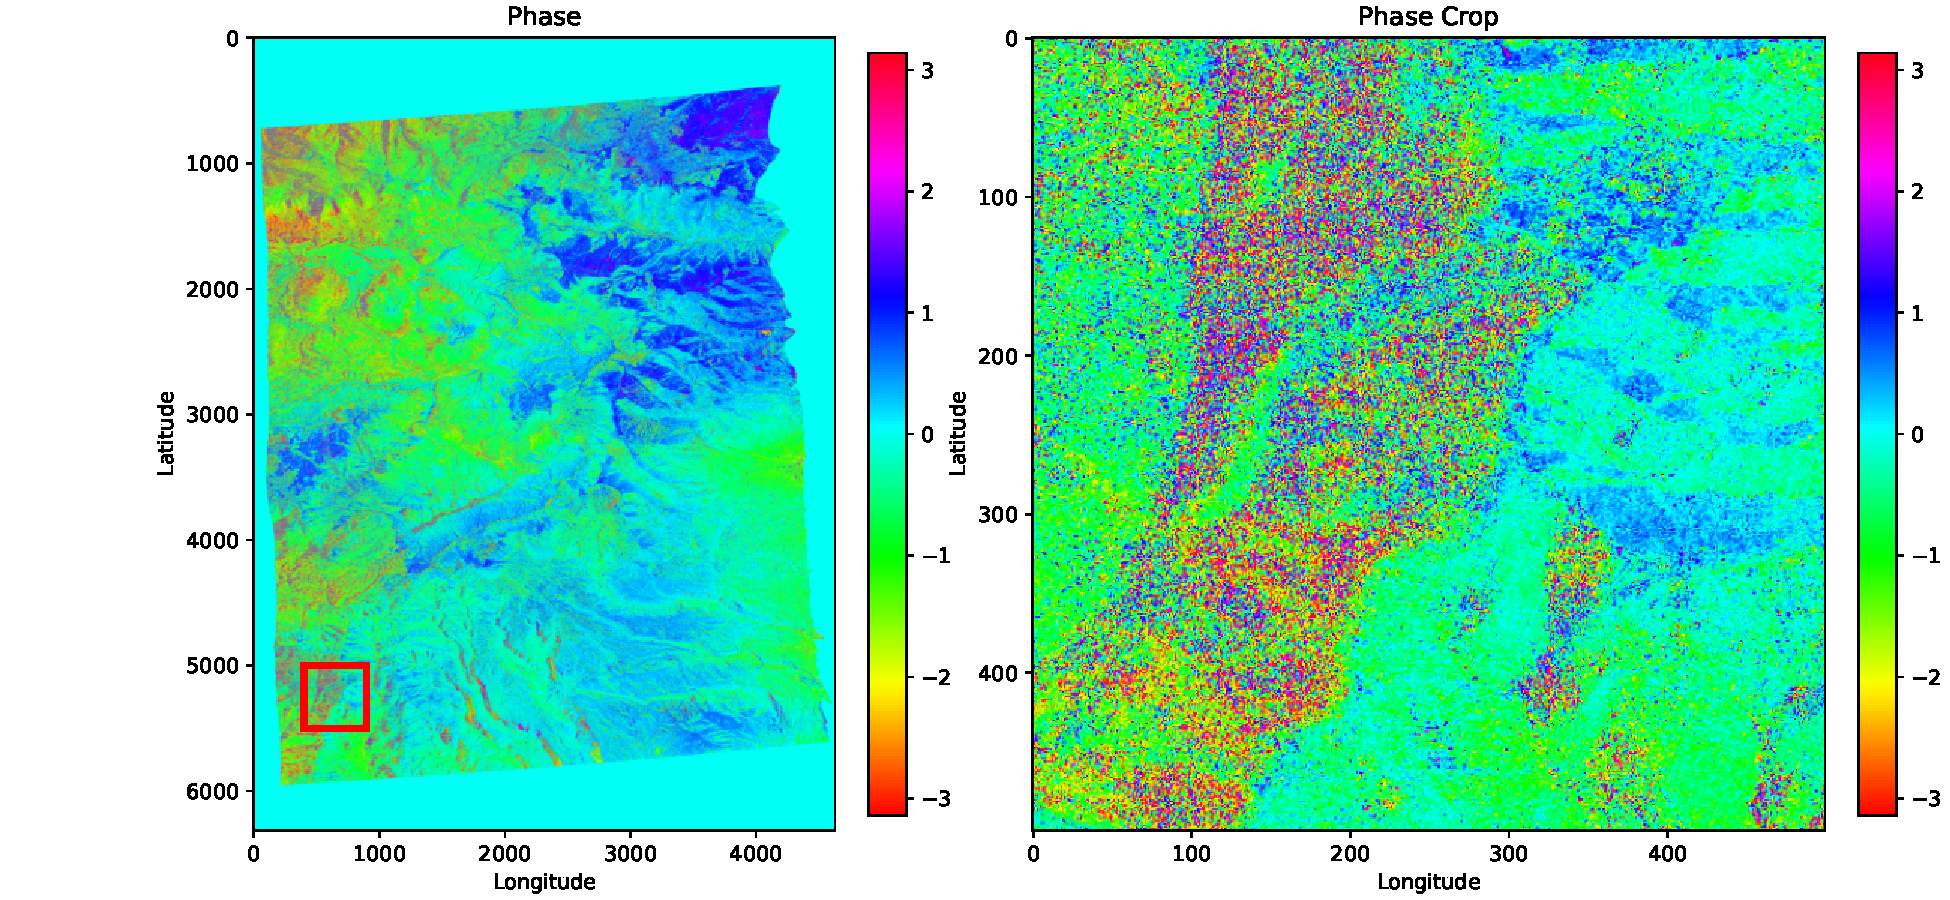
\includegraphics[width=1.0\linewidth]{los_alamos_orig_and_crop_500}
     %DIF > }
    \caption{\DIFaddFL{Interferometric phase images acquired by the UAVSAR sensor: (a) Los Alamos, USA; (b) Los Alamos ROI .}}
     \label{fig:insar_uavsar_los_alamos} 
\end{figure}

\DIFaddend \subsubsection{Robledo Volcano InSAR Image}\label{subsec:materials_robledo}

%From the same source, we obtained the Robledo Volcano InSAR image, Argentina. 
Figure~\DIFdelbegin \DIFdel{\ref{fig:insar_uavsar_robledo:b} }\DIFdelend \DIFaddbegin \DIFadd{\ref{fig:insar_uavsar_robledo} }\DIFaddend shows the InSAR image of Robledo Volcano, Argentina, to the left, while the ROI is shown to the right.


\begin{figure}[hbt]
    \DIFdelbeginFL %DIFDELCMD < \centering
%DIFDELCMD <          \subfloat[Los Alamos InSAR Image \label{fig:insar_uavsar_los_alamos:a}]{%
%DIFDELCMD < %       \includegraphics[width=0.52\linewidth]{arquivo_fix_alamos.pdf}
%DIFDELCMD < 		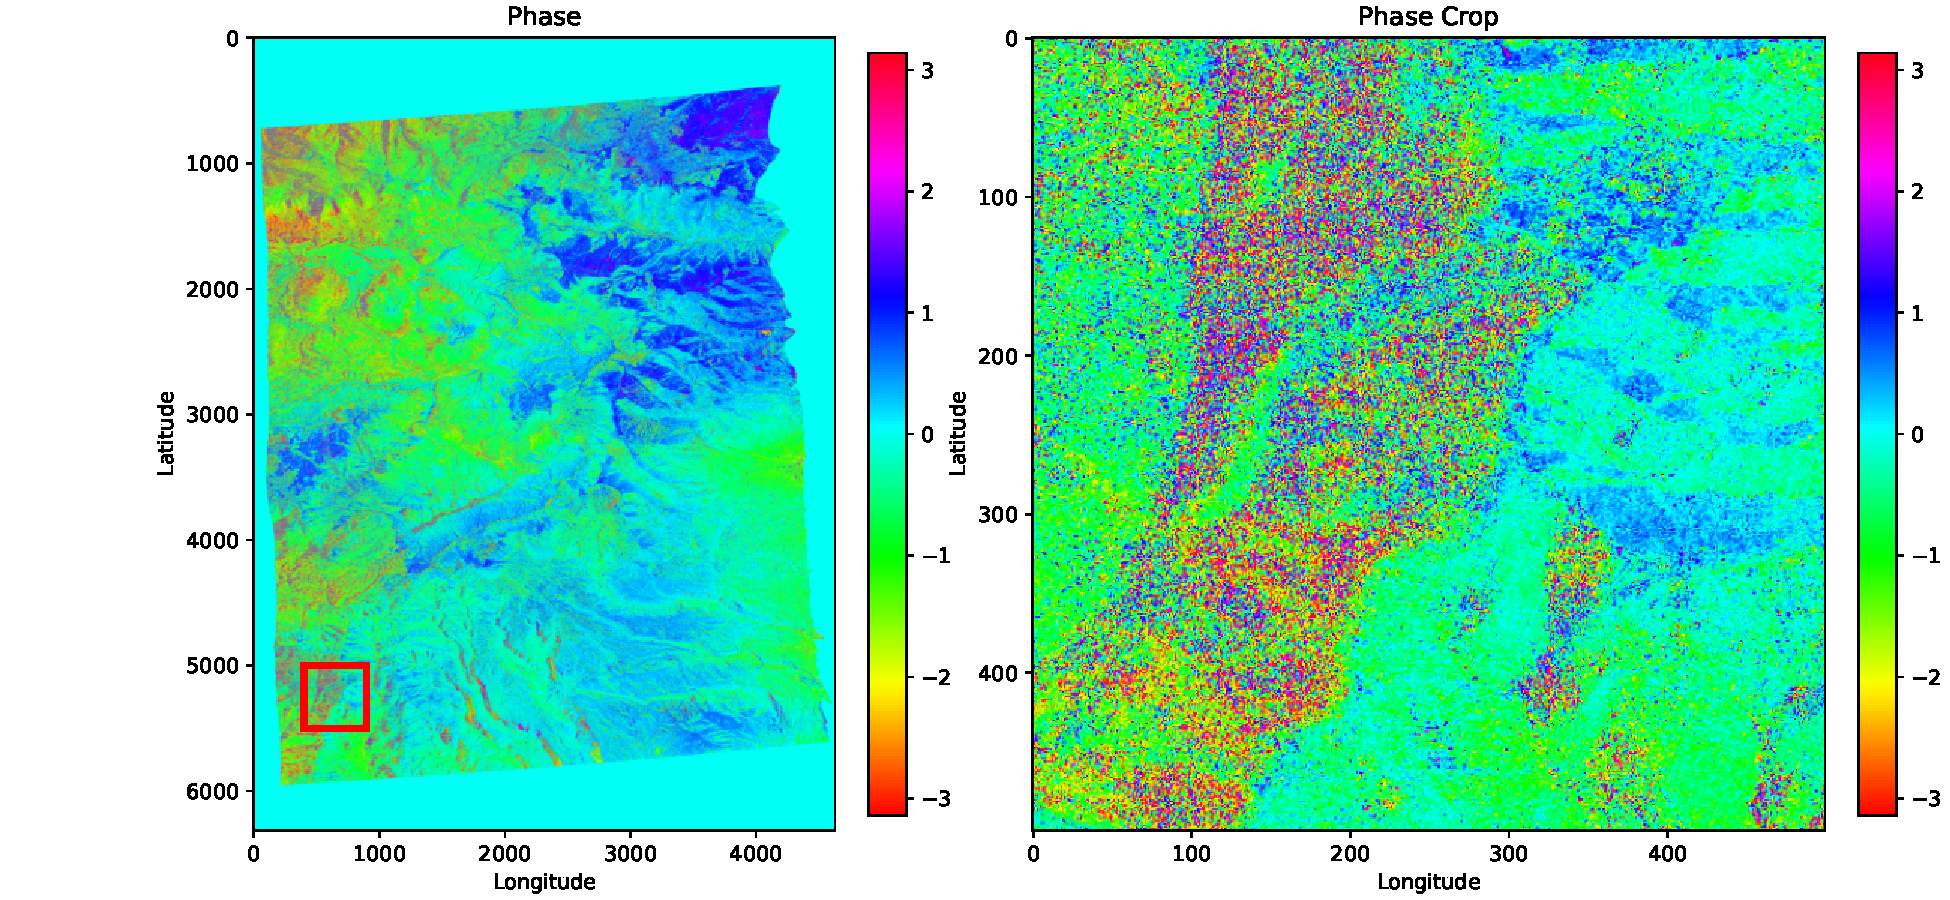
\includegraphics[width=1.0\linewidth]{los_alamos_orig_and_crop_500}
%DIFDELCMD <      }\\
%DIFDELCMD <      \subfloat[Robledo Volcano InSAR Image  \label{fig:insar_uavsar_robledo:b}]{%
%DIFDELCMD < %       \includegraphics[width=0.51\linewidth]{arquivo_fix_robledo.pdf}
%DIFDELCMD <        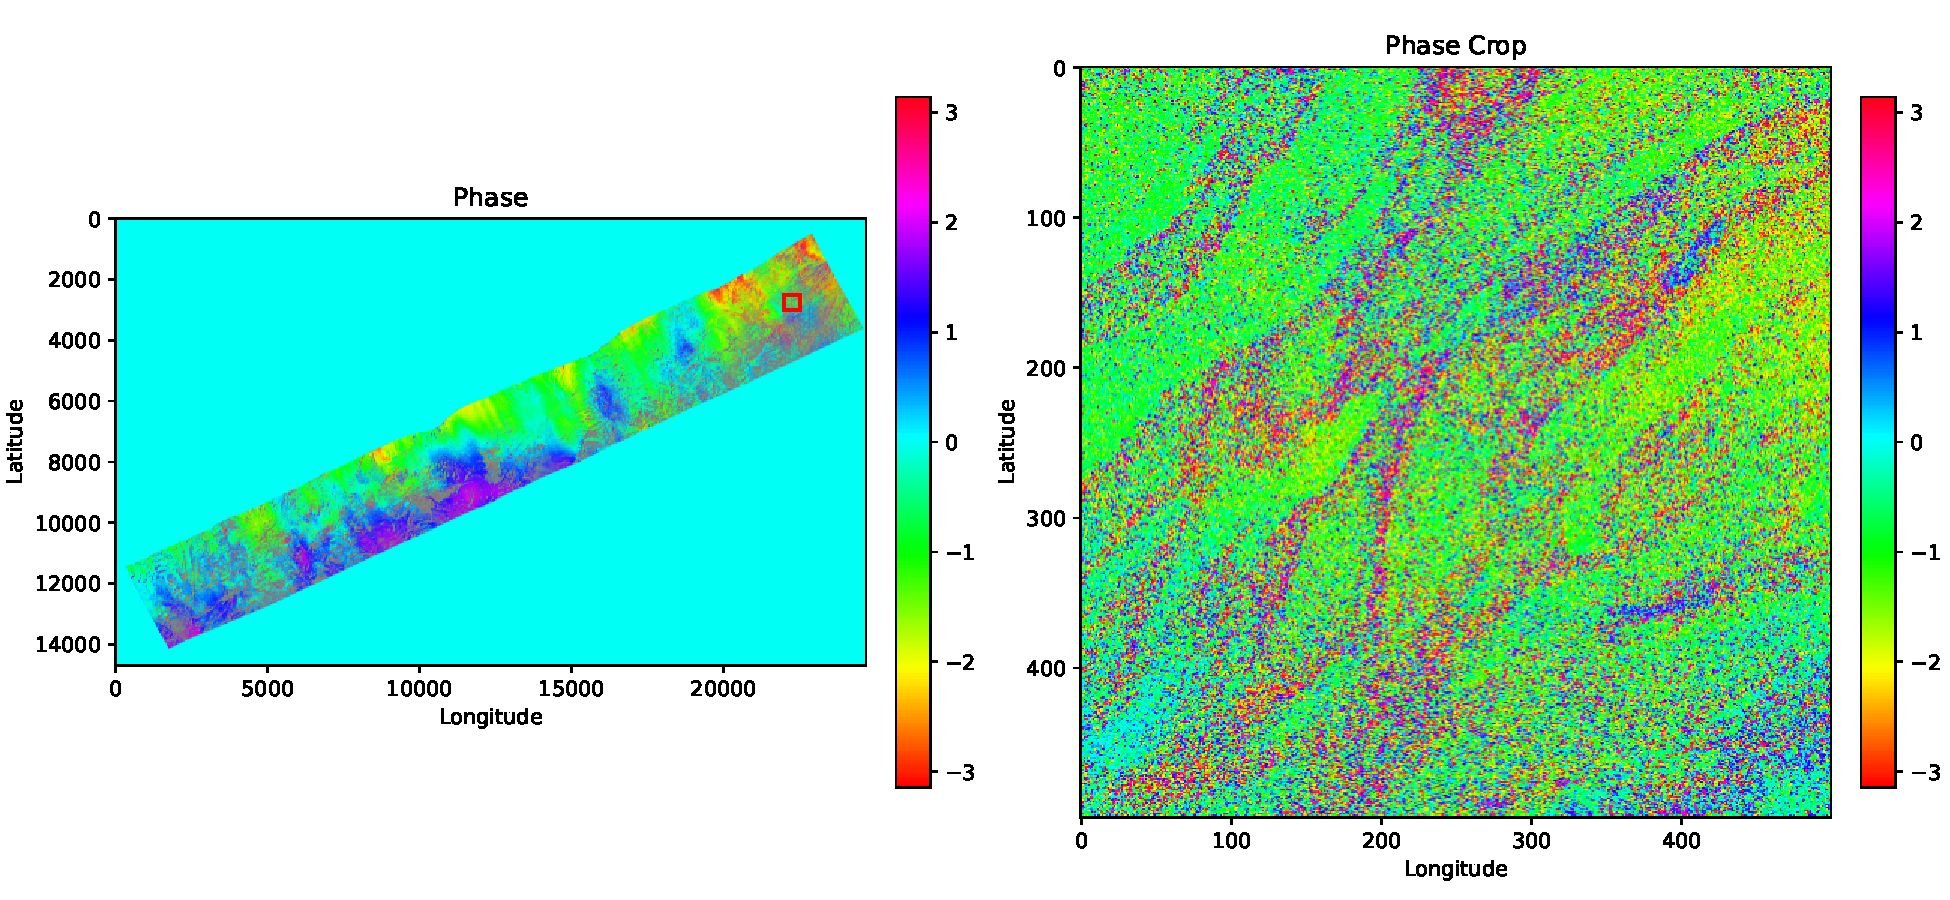
\includegraphics[width=1.0\linewidth]{robledo_orig_and_crop_500}
%DIFDELCMD <      }
%DIFDELCMD <     %%%
\DIFdelendFL %DIF > \centering
     %DIF > \subfloat[Robledo Volcano InSAR Image  \label{fig:insar_uavsar_robledo:b}]{%
%DIF >        \includegraphics[width=0.51\linewidth]{arquivo_fix_robledo.pdf}
       \DIFaddbeginFL 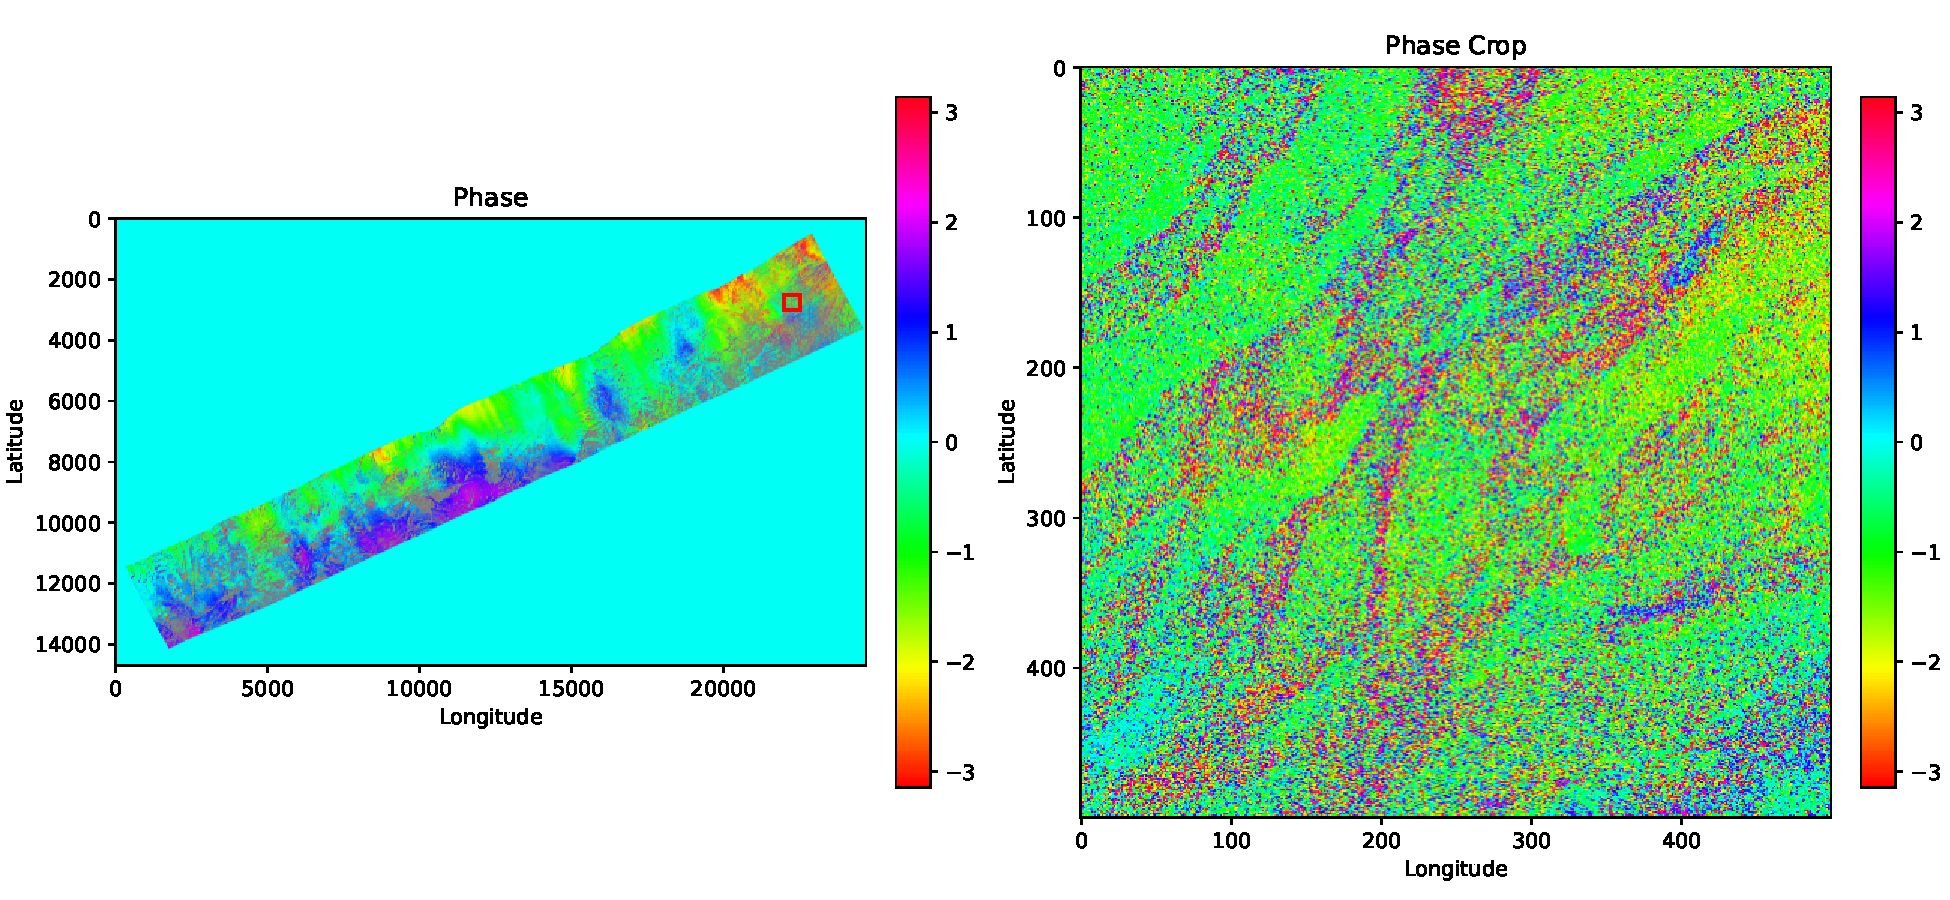
\includegraphics[width=1.0\linewidth]{robledo_orig_and_crop_500}
     %DIF > }
    \DIFaddendFL \caption{Interferometric phase images acquired by the UAVSAR sensor: (a) \DIFdelbeginFL \DIFdelFL{Los Alamos}\DIFdelendFL \DIFaddbeginFL \DIFaddFL{Robledo Volcano}\DIFaddendFL , \DIFdelbeginFL \DIFdelFL{USA}\DIFdelendFL \DIFaddbeginFL \DIFaddFL{Argentina}\DIFaddendFL ; (b) Robledo \DIFdelbeginFL \DIFdelFL{Volcano, Argentina.}\DIFdelendFL \DIFaddbeginFL \DIFaddFL{ROI}\DIFaddendFL }
     \DIFdelbeginFL %DIFDELCMD < \label{fig:insar_uavsar} 
%DIFDELCMD < %%%
\DIFdelendFL \DIFaddbeginFL \label{fig:insar_uavsar_robledo} 
\DIFaddendFL \end{figure}
\DIFaddbegin \newpage
\DIFaddend 


%%%%%%%%%%%%%%%%%%%%%%%%%%%%%%%%%%%%%%%%%%%%%%%%%%%%%%%%%%%%%%%%%%%%%%%%%%%%%%%%%%
%%%%%%%%%%%%%%%%%%%%%%%%%%% Comment #8 %%%%%%%%%%%%%%%%%%%%%%%%%%%%%%%%%%%%%%%%%%%
%%%%%%%%%%%%%%%%%%%%%%%%%%%%%%%%%%%%%%%%%%%%%%%%%%%%%%%%%%%%%%%%%%%%%%%%%%%%%%%%%%
\vskip3em\begin{tcolorbox}[colback=red!5!white,colframe=red!75!black,title=Comment 8]
8. In Figure 10-12, d) TcNfilter should be (d).
\end{tcolorbox}

\begin{tcolorbox}[colback=white,colframe=black,title=Changes 8]
Yes, of course, thank you a lot.
\end{tcolorbox}

\bibliographystyle{abbrvnat}

%Sets the bibliography style to UNSRT and imports the 
%bibliography file "sample.bib".
\bibliography{bibliografia1}
\end{document}